% Capítulo 6 (Resultados) — Slide 10 — Sensibilidade do CTI ajustado (figura isolada)
\begin{frame}{CTI ajustado por estabilidade}
  \centering
  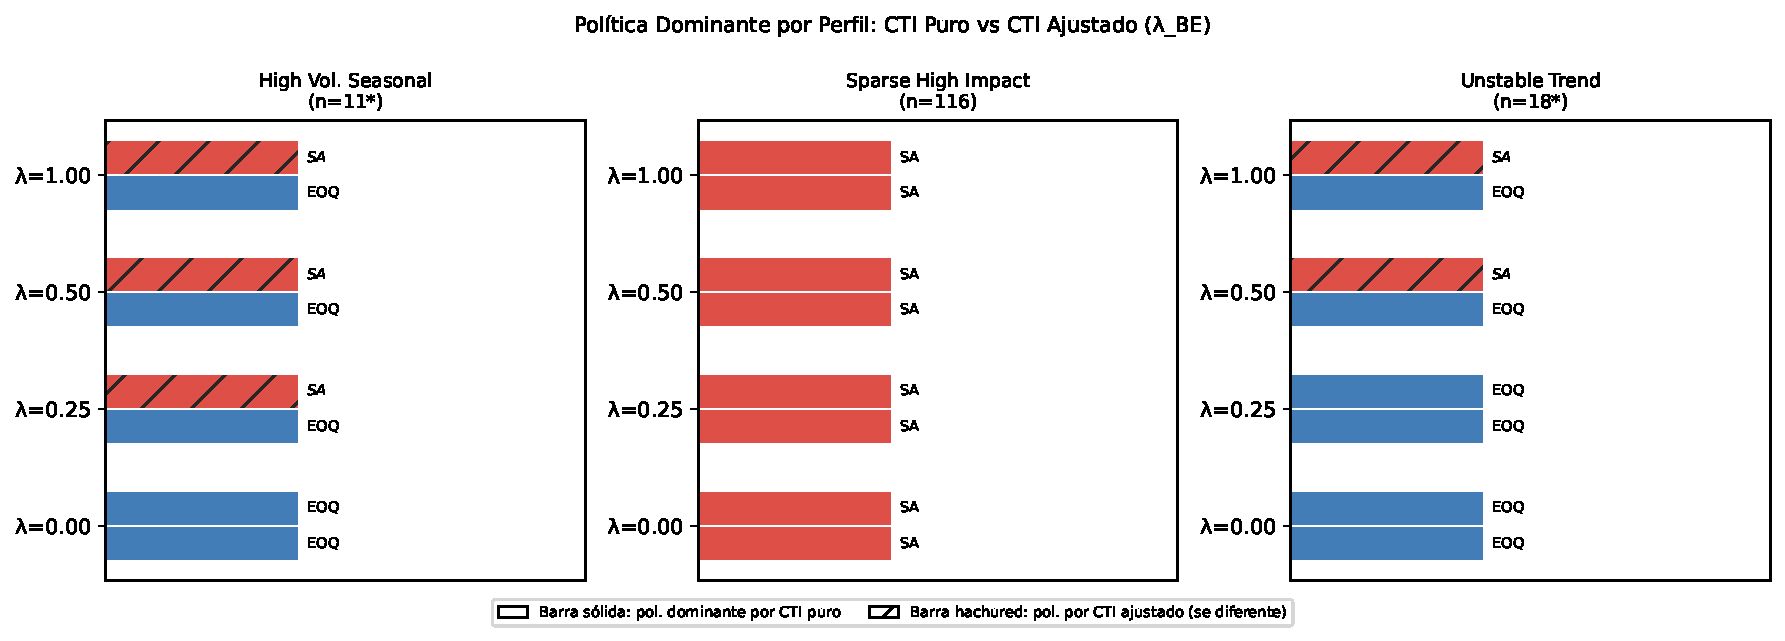
\includegraphics[width=0.95\linewidth,height=6.0cm,keepaspectratio]{figures/cti_adjusted_sensitivity.pdf}\\[0.4em]
  {\small Sensibilidade do critério ajustado $J(\pi,g)$ ao peso $\lambda_{BE}$ (análise complementar).}
  \note{
    Este gráfico mostra como a política única ótima migra conforme o peso
    da penalidade por instabilidade aumenta. Com lambda zero, o critério
    recupera exatamente o CTI puro, em que o EOQ domina. A partir de lambda
    igual a 0,25, a política única de menor critério ajustado passa a ser o
    SA, que é muito mais estável que o EOQ. Essa transição é o ponto
    principal da figura: a política preferida depende explicitamente de
    quanto se valoriza estabilidade dos pedidos frente a custo puro.
  }
\end{frame}
